\chapter{Dataset and Preprocessing}
\label{chap:dataset}

This chapter describes the dataset, the preprocessing pipeline, and the experimental splits used for both standard classification and zero-day attack detection.

% ============================================================
\section{The ToN\_IoT Dataset}
\label{sec:toniot}

I use the ToN\_IoT dataset~\cite{toniot2020dataset}, captured from an IoT testbed at UNSW. Specifically, I work with \texttt{Network\_dataset\_11}: 1,000,000 flow records over 46~columns combining transport-layer metadata (ports, protocol, duration, byte and packet counts), application-layer fields (DNS, HTTP, SSL), and a traffic class label.

The dataset contains three classes: \emph{normal} traffic (35,168 samples, 3.5\%), \emph{DoS} attacks (839,637 samples, 84.0\%), and \emph{injection} attacks (125,195 samples, 12.5\%).

% ============================================================
\section{Feature Selection and Cleaning}
\label{sec:cleaning}

Of the 46~original columns, 21 are constant across all records (SSL, HTTP, and miscellaneous fields uniformly \texttt{'-'} or~0) and carry no information. I also drop capture-specific identifiers (\texttt{ts}, \texttt{src\_ip}, \texttt{dst\_ip}) that would not generalize, the text-valued \texttt{dns\_query}, and the redundant binary \texttt{label}. This leaves 19~features (see Table~\ref{tab:features} in Appendix~\ref{app:full_results}).

To reduce dimensionality for quantum encoding, I first perform the train/test split (Section~\ref{sec:splits}), then---using the training set only, to avoid data leakage~\cite{kapoor2023leakage}---compute pairwise Pearson correlations and drop features with correlation above 0.95, rank the rest by ANOVA F-score, and keep the top~8 to match the qubit count. The same features are then applied to the test set without refitting. Figure~\ref{fig:feature_importance} shows the ranking; the selected features are \texttt{src\_port}, \texttt{service}, \texttt{dst\_port}, \texttt{conn\_state}, \texttt{src\_pkts}, \texttt{src\_ip\_bytes}, \texttt{proto}, and \texttt{dns\_AA}.

\begin{figure}[ht]
    \centering
    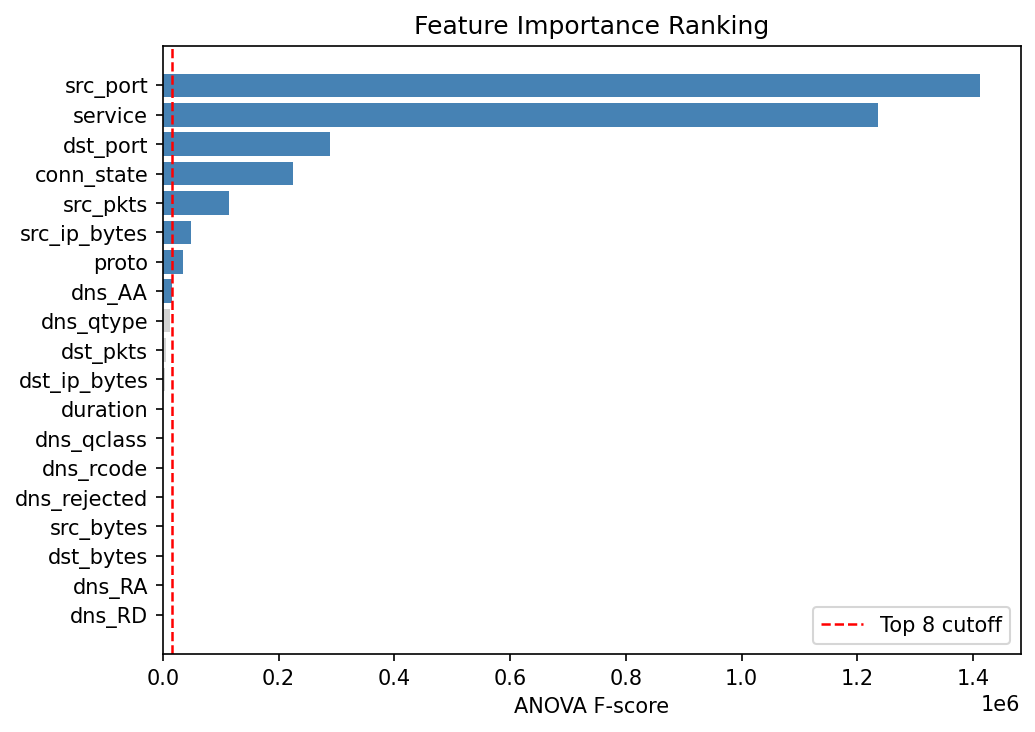
\includegraphics[width=0.75\textwidth]{figures/feature_importance.png}
    \caption{ANOVA F-score ranking of the 19 candidate features. The top~8 (blue) are selected for quantum encoding; the red dashed line marks the cutoff.}
    \label{fig:feature_importance}
\end{figure}

% ============================================================
\section{Handling Class Imbalance}
\label{sec:imbalance}

The severe class imbalance is problematic for training. Interpolation-based augmentation (e.g., SMOTE) is unsuitable here: a linear mix of two flows with different TCP flags or connection states produces a flow that cannot exist in practice. I instead use \emph{random undersampling} of the majority classes to match the minority (35,168~per class), giving a balanced dataset of 105,504~samples; quantum experiments subsample further due to simulation cost.

% ============================================================
\section{Normalization and Experimental Splits}
\label{sec:splits}

For angle encoding (Section~\ref{sec:qcnn}), each feature is scaled to $[0, \pi]$ via min-max normalization:
\begin{equation}
    x_i^{\text{scaled}} = \pi \cdot \frac{x_i - \min x_i}{\max x_i - \min x_i},
\end{equation}
so each feature spans the full range of a rotation gate. The scaler is fit on the training set only.

I define two experimental settings:

\textbf{Standard classification.} The balanced dataset is split 80/20 with stratified sampling (84,403 training / 21,101 test). All models share the same splits.

\textbf{Zero-day attack detection.} The model is trained on normal and DoS traffic only, then evaluated on injection attacks absent from training---simulating an unseen attack type (Figure~\ref{fig:zeroday_split}).

For quantum experiments, the standard 3-class split is stratified-subsampled to 500~training samples and 200~test samples, since circuit simulation on classical hardware scales linearly with dataset size. The zero-day quantum split uses fixed (non-stratified) random subsamples of the same size from the normal+DoS training set and the injection-only test set.

\begin{figure}[ht]
\centering
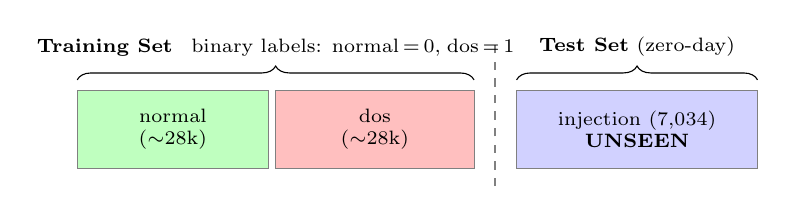
\begin{tikzpicture}[scale=0.9]
    % Training boxes
    \fill[green!25] (0,   0) rectangle (2.7, 1.1);
    \draw[gray]     (0,   0) rectangle (2.7, 1.1);
    \fill[red!25]   (2.8, 0) rectangle (5.6, 1.1);
    \draw[gray]     (2.8, 0) rectangle (5.6, 1.1);
    % Test box
    \fill[blue!18]  (6.2, 0) rectangle (9.6, 1.1);
    \draw[gray]     (6.2, 0) rectangle (9.6, 1.1);
    % Dashed separator
    \draw[dashed, thick, gray] (5.9, -0.25) -- (5.9, 1.85);
    % Labels inside boxes (two lines each)
    \node[align=center, font=\scriptsize] at (1.35, 0.55) {normal\\($\sim$28k)};
    \node[align=center, font=\scriptsize] at (4.2,  0.55) {dos\\($\sim$28k)};
    \node[align=center, font=\scriptsize] at (7.9,  0.55) {injection (7{,}034)\\\textbf{UNSEEN}};
    % Top braces
    \draw[decorate, decoration={brace,amplitude=5pt}] (0, 1.25) -- (5.6, 1.25)
        node[midway, above=5pt, font=\scriptsize]
        {\textbf{Training Set} \enspace binary labels: normal\,=\,0,\;dos\,=\,1};
    \draw[decorate, decoration={brace,amplitude=5pt}] (6.2, 1.25) -- (9.6, 1.25)
        node[midway, above=5pt, font=\scriptsize]
        {\textbf{Test Set} (zero-day)};
\end{tikzpicture}
\caption{Zero-day experimental split. The model trains on normal and DoS traffic only (binary classification), then is tested on injection attacks --- an entirely unseen class. High detection rate indicates genuine generalization beyond memorized attack patterns.}
\label{fig:zeroday_split}
\end{figure}
